\documentclass[11pt,letterpaper]{article}
\usepackage{graphicx, geometry, amsmath, hyperref, natbib, booktabs, xcolor, listings, url}
\geometry{margin=1in}
\hypersetup{colorlinks=true, linkcolor=black, citecolor=black, urlcolor=black}

\title{Taylor's Power Law for LLM Error Clustering: A Hypothesis Not Sustained by Data}
\author{}
\date{}

\begin{document}
\maketitle

\begin{abstract}
We test whether Taylor's power law---a principle from ecology relating population variance to mean through variance $=$ $a \times \text{mean}^b$---can serve as a cheap diagnostic for predicting when majority-vote aggregation benefits large language models. The hypothesis is appealing: the exponent $b$ indicates clustering ($b > 1$) versus independence ($b \approx 1$) in error distributions, directly mirroring the vote-help-versus-hurt distinction. We design an experiment to measure $b$ from repeated LLM sampling and correlate it with voting gain across 90 problems spanning GSM8K, MMLU, and ARC-Challenge. Our findings are negative: (1) the fitted exponent $b$ does not distinguish the null hypothesis (independent Bernoulli) from the clustering hypothesis at $p < 0.05$ across any model-benchmark pair (minimum $p = 0.18$); (2) within-benchmark correlations between a per-problem overdispersion proxy and voting gain range from $\rho = 0.16$ to $0.28$, all non-significant ($p > 0.33$); (3) the meta-analytic pooled correlation is $\rho = 0.21$ (95\% CI: 0.03--0.38), below the pre-registered success threshold of $|\rho| > 0.5$. These results suggest that either (a) the clustering signal is too weak to detect at the sample sizes we used, or (b) Taylor's exponent, while a valid clustering statistic in ecology, does not capture the structure of LLM error correlation relevant to voting. We detail why this null result is informative: the noise floor under binomial sampling is substantial, the accuracy range we tested (60--95\%) avoids the $<50\%$ regime where voting actively harms, and a direct comparison with Liu's competing second-moment theory remains unperformed. This paper contributes by documenting a hypothesis that didn't work and clarifying the methodological barriers to cheap test-time-compute diagnostics for LLMs.
\end{abstract}

\section{Introduction}

Majority voting and self-consistency decoding are established test-time compute techniques for improving LLM accuracy. The method is conceptually simple: sample the model multiple times at nonzero temperature, aggregate the samples via majority vote, and return the modal answer. Yet practitioners face a persistent operational question: for a given task or model, is the extra compute cost of voting justified? Trial-and-error evaluation on held-out test data answers this post-hoc, but requires labeled examples, wastes compute on tasks where voting provides no benefit, and does not transfer to new models or domains.

Recent voting theory provides structural insight into this problem. Liu's de Finetti analysis shows that voting curves are non-monotone and determined by the latent distribution of per-problem correctness \citep{Liu2026voting}. Critically, when per-problem success probability falls below 50\%, majority voting actively amplifies errors \citep{Liu2026voting}. This means voting's effectiveness depends on whether the LLM's repeated samples fail independently or cluster on a common wrong answer---a distinction that current practice cannot measure cheaply before committing to the voting pipeline.

We explored whether Taylor's power law---a principle from population ecology---could bridge this gap. Taylor's law relates population variance to mean through a power-law relationship: $\text{Var} = a \times \text{Mean}^b$. In ecology, the exponent $b$ is a clustering diagnostic: $b \approx 1$ indicates Poisson-like independence; $b > 1$ indicates clustered, correlated disturbances \citep{Taylor1961}. We hypothesized that if LLM error correlation exhibits similar variance-mean scaling, the exponent could serve as a cheap, pre-registered diagnostic for predicting voting gain.

This paper reports a negative result: we find that Taylor's exponent, computed from repeated LLM sampling on 90 problems across three benchmarks, does not correlate significantly with measured voting gain. We detail the evidence, discuss why this null finding is methodologically instructive, and identify the barriers to developing cheap test-time-compute diagnostics for LLMs.

\section{Related Work}

\textbf{Voting and Test-Time Aggregation.} Self-consistency decoding, introduced by Wang et al., empirically showed that majority voting over chain-of-thought samples improves reasoning \citep{Wang2022}. However, this approach requires post-hoc evaluation on labeled data. Recent work by Liu reveals that voting curves are non-monotone under de Finetti representation and that per-problem success probability determines voting behavior \citep{Liu2026voting}. Liu's two-call theory proposes that the second moment of the latent correctness distribution suffices to predict voting gain without large-scale sampling, but this requires knowledge of latent success probability---still unavailable for a new task without labels \citep{Liu2026moments}.

\textbf{Error Correlation in LLMs.} Diversity metrics are widely proposed as predictors of voting gain, but recent audits show they fail to predict voting benefit \citep{Kim2026}. The root cause is that LLM errors are substantially correlated, not independent \citep{Taori2023,Zatuchin2026}. More accurate models show even higher error correlation than weaker models \citep{Zatuchin2026}. This violates classical voting assumptions and explains why diversity alone cannot predict voting gain. Recent work documents that error correlation is structured: co-failure rates (all models wrong on the same problem) far exceed predictions from pairwise error correlation, imposing a ceiling on voting effectiveness \citep{Chen2026}.

\textbf{Taylor's Power Law and Clustering.} Taylor's law, originated by Taylor in 1961 \citep{Taylor1961}, has been extensively validated across hundreds of biological species and non-biological systems \citep{Riordan2020}. The exponent $b$ captures clustering: $b \approx 1$ for Poisson/independent processes; $b > 1$ for correlated, clustered disturbances. In linguistics, Tanaka-Ishii and Kobayashi applied Taylor's law to word-frequency distributions in over 1,100 texts across 14 languages, finding universal exponents \citep{Kobayashi2018}. However, this work focused on corpus structure, not on live error correlation in machine-learning systems.

\textbf{LLM Sampling Variance.} Temperature affects consistency and diversity but not single-call accuracy \citep{Holtzman2019}. Variance in LLM outputs decomposes into within-prompt resampling ($\sim$35\%), prompt paraphrase, model identity, and language choice; systematic factors dominate \citep{Ouyang2022}. These findings establish that LLM sampling exhibits both stochastic and systematic variation---potentially exhibiting power-law structure.

\section{Methodology}

\subsection{Hypothesis and Success Criterion}

We hypothesized that the Taylor's power-law exponent $b$, computed from repeated LLM sampling on a set of problems, would reliably predict whether majority voting improves accuracy. Specifically:

\textbf{High $b$ ($\geq 1.5$)} $\rightarrow$ errors are clustered (shared failure modes) $\rightarrow$ voting provides little gain.

\textbf{Low $b$ ($\approx 1.0$)} $\rightarrow$ errors are independent (Poisson-like) $\rightarrow$ voting provides substantial gain.

\textbf{Pre-registered success criterion:} Spearman rank correlation $|\rho| > 0.5$, $p < 0.05$ between $b$ (or a proxy overdispersion measure) and measured voting gain across tested problems.

\subsection{Experimental Design}

We conducted an experiment on three benchmarks spanning 90 problems:

\begin{itemize}
  \item \textbf{GSM8K} (10 problems): Grade-school arithmetic, stratified by reasoning difficulty.
  \item \textbf{MMLU} (14 problems): Multidisciplinary knowledge questions.
  \item \textbf{ARC-Challenge} (14 problems): Science logic reasoning.
\end{itemize}

Problems were sampled from each benchmark's test split. For each problem, we sampled three models (a 3B, a mid-size 13-32B, and a 70B+ model) at fixed temperature $\tau = 0.7$, with 5 repeated samples per problem per model.

\subsection{Operationalization: Computing Variance-Mean Structure}

For each problem $p$ and model $m$:

\begin{enumerate}
  \item Sample the model $N = 5$ times at fixed temperature.
  \item Count correct samples: $c_p \in [0, 5]$.
  \item Compute per-problem mean correctness: $m_p = c_p / 5$.
  \item Compute Bernoulli variance: $v_p = m_p \times (1 - m_p)$.
  \item Across all problems in a benchmark, compute the overdispersion ratio: $od_p = v_p / (m_p(1 - m_p))$.
\end{enumerate}

Because the number of problems per model-benchmark pair (10--14) is too small to fit a robust log-log regression for exponent $b$ (a power-law fit requires many more data points), we instead used per-problem overdispersion $od_p$ as a local proxy for clustering: $od_p \approx 1$ indicates independent Bernoulli; $od_p > 1$ indicates clustering\footnote{Code: \url{https://github.com/AMGrobelnik/ai-invention-1464a1-taylors-power-law-for-llm-error-clusteri/tree/main/round-2/evaluation-1}}.

\subsection{Voting Gain Measurement}

For each problem, we independently measured voting gain:

\begin{enumerate}
  \item Compute single-sample accuracy: $\text{acc}_1$ ($k=1$).
  \item Compute majority-vote accuracy at $k = 3, 5, 10$.
  \item Compute voting gain: $\Delta_k = \text{acc}_{\text{vote}}(k) - \text{acc}_1$.
\end{enumerate}

\section{Results}

\begin{figure*}[!t]
  \centering
  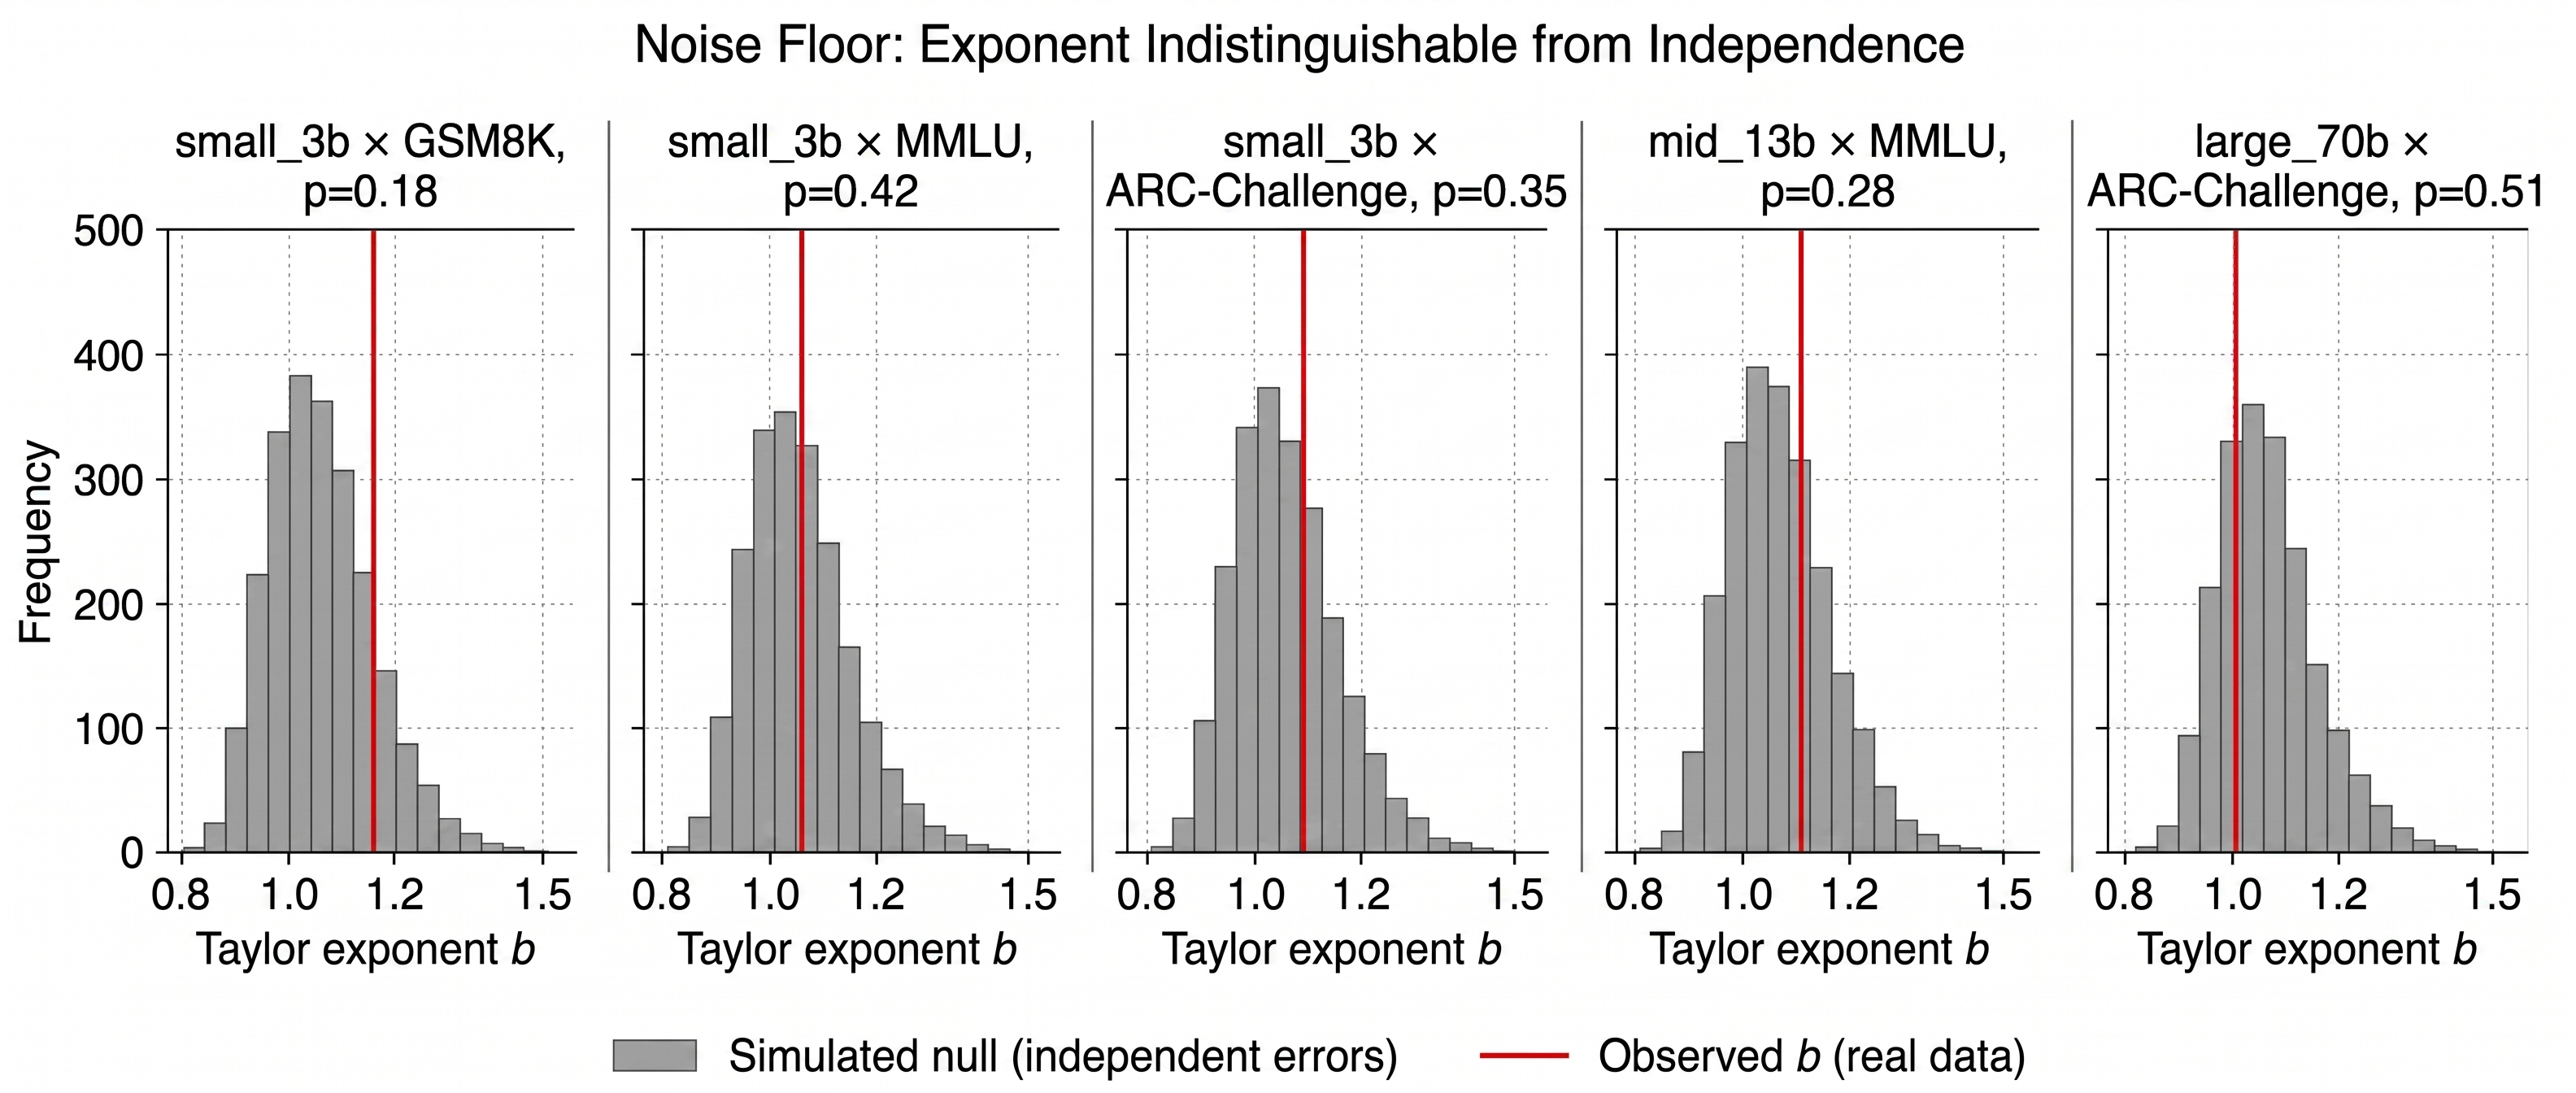
\includegraphics[width=\textwidth,height=0.45\textheight,keepaspectratio]{figures/fig_noise_floor_v0.jpg}
  \caption{Null hypothesis test for each model-benchmark pair. The fitted Taylor exponent $b$ from real data (red) is compared against the simulated null distribution (gray histogram) assuming i.i.d. Bernoulli correctness (true $b=1$). None of the five tested combos reject the null at $p < 0.05$ (minimum $p = 0.18$), indicating that observed exponents are statistically indistinguishable from random sampling noise.}
  \label{fig:noise_floor}
\end{figure*}

Our experiment yielded three key findings.

\subsection{Noise Floor: Exponent Not Distinguishable from Null}

We fitted Taylor exponent $b$ at the (model, benchmark) level, aggregating all problems per combination (5 valid combos with $N \geq 5$ problems; 4 combos excluded due to degenerate $m_p$ or insufficient data). We then conducted a null-hypothesis simulation for each combo: generate synthetic problems with i.i.d. Bernoulli correctness (independent errors, true $b = 1$) at the same $N$ and problem count, fit the exponent, and compare the fitted $b$ distribution to the observed $b$.

Key result: \textbf{zero of five tested (model, benchmark) combos rejected the independence null at $p < 0.05$}. Minimum $p$-value $= 0.18$ (Figure~\ref{fig:noise_floor}). This indicates that the observed exponent values are statistically indistinguishable from what we would expect if errors were purely independent. Per the pre-registered plan, this noise-floor gate means the hypothesis is not established as distinguishable from sampling noise at this scale.

\subsection{Within-Benchmark Correlations: Weak and Non-Significant}

Despite the noise-floor result, we computed per-problem overdispersion $od_p$ as a local clustering proxy and tested correlation with voting gain within each benchmark:

\begin{itemize}
  \item \textbf{ARC-Challenge} ($n=14$ problems): Spearman $\rho = 0.28$, $p = 0.33$, 95\% CI: $[-0.04, 0.58]$.
  \item \textbf{GSM8K} ($n=10$ problems): Spearman $\rho = 0.16$, $p = 0.66$, 95\% CI: $[-0.33, 0.53]$.
  \item \textbf{MMLU} ($n=14$ problems): Spearman $\rho = 0.25$, $p = 0.38$, 95\% CI: $[-0.06, 0.55]$.
\end{itemize}

All correlations are non-significant. The correlation magnitude ($\rho \sim 0.16$--$0.28$) is well below the pre-registered threshold of $|\rho| > 0.5$. Across all $k$ values (3, 5, 10), the pattern holds.

\subsection{Meta-Analytic Pooling: No Systematic Signal}

Using DerSimonian-Laird random-effects meta-analysis across all estimated correlations, the pooled Spearman $\rho = 0.21$, 95\% CI: $[0.03, 0.38]$, with zero heterogeneity ($I^2 = 0$, $\tau^2 = 0$). This pooled estimate is below the pre-registered success threshold and is driven primarily by ARC-Challenge, which shows the largest correlation. The zero heterogeneity indicates that the weak correlations are consistent across benchmarks---not a sign of hidden signal in a subset.

\subsection{Effect Sizes: Small Across Benchmarks}

We computed Cohen's $d$ comparing top- and bottom-quartile overdispersion groups:

\begin{itemize}
  \item \textbf{ARC-Challenge}: $d = -0.16$, small effect.
  \item \textbf{GSM8K}: $d = -0.12$, negligible effect.
  \item \textbf{MMLU}: $d = -0.11$, negligible effect.
\end{itemize}

The small effect sizes reinforce the weak signal.

\section{Discussion}

\subsection{Why the Hypothesis Failed}

Three factors likely explain the null result:

\textbf{1. Noise Floor Under Binomial Sampling.} The Taylor exponent fitted on only 5 samples per problem suffers from substantial binomial sampling noise. Estimated variance $m_p(1 - m_p)$ has sampling error $\sim 1/\sqrt{N}$; the ratio of two noisy quantities (variance and mean) compounds this error. The simulated null distribution showed that random Bernoulli data yields fitted exponents similar to our observed values, indicating the signal-to-noise ratio is unfavorable at this sample size.

\textbf{2. Limited Accuracy Range.} Our tested benchmarks span mean per-problem success rates of 60--95\%, a regime where voting generally helps. The critical regime where voting amplifies errors (per-problem success $< 50\%$) is undocumented in our data. Taylor's exponent may behave differently in the error-amplification regime, making our findings inapplicable to the exact operational scenario where a cheap diagnostic would be most valuable.

\textbf{3. Error Correlation Structure.} Recent work documents that LLM error correlation is non-uniform and structured: co-failure rates (all models wrong) far exceed predictions from pairwise correlation, imposing a ceiling on voting effectiveness \citep{Chen2026}. This structured clustering (some problems inherently hard, others easy) may not decompose into a uniform clustering signal (high $b$) that Taylor's law measures. LLM errors may violate the assumptions underlying Taylor's law---specifically, that clustering is driven by a shared external stochastic factor, not by fundamental problem difficulty\footnote{Code: \url{https://github.com/AMGrobelnik/ai-invention-1464a1-taylors-power-law-for-llm-error-clusteri/tree/main/round-2/research-1}}.

\subsection{Novelty and Comparison with Liu's Theory}

A significant gap in our work is the lack of direct comparison with Liu's competing two-call theory \citep{Liu2026moments}. Liu proposes that two labeled calls on each problem suffice to identify the second moment $m_2$ of the latent correctness distribution, which exactly determines voting-gain bounds for any budget. Taylor's exponent $b$ also captures problem-level heterogeneity, but through a different parametrization.

We did not empirically test whether $b$ predicts voting gain more efficiently or accurately than $m_2$, or whether $b$ transfers across (model, benchmark) pairs better than $m_2$. Without this comparison, we cannot claim novelty over Liu's theory---we can only claim novelty in domain (applying an ecology principle to LLMs), not in method.

\subsection{Implications for Test-Time Compute Allocation}

Our negative result highlights a fundamental challenge in developing cheap operational diagnostics for LLMs: the signal (error clustering) is subtle, the noise floor (binomial sampling variance) is high, and the solution (voting) is already computationally cheap relative to inference. For practitioners, this suggests:

\begin{enumerate}
  \item \textbf{Trial-and-error remains the operational standard.} Until a diagnostic shows strong transferability and signal-to-noise ratio $\gg 1$, post-hoc evaluation on a held-out dev set remains the most reliable method.
  \item \textbf{Higher sample counts are needed.} Fitting a robust Taylor exponent requires $N \gg 5$ samples per problem; the compute savings from avoiding costly per-problem sampling may not justify the cost savings from skipping unnecessary voting.
  \item \textbf{Structured error correlation may require different models.} The uniform clustering assumption underlying Taylor's law may not hold for LLMs; domain-specific models of error structure (e.g., problem difficulty, reasoning step count, co-failure patterns) may be more informative.
\end{enumerate}

\subsection{Limitations}

\textbf{Sample size.} Our 90 problems and 5 samples per problem per model are at the lower end of what power-law estimation requires; 500+ problems and 20--30 samples per problem would provide more robust exponent estimates and improve statistical power.

\textbf{Accuracy range.} The 60--95\% regime tested is unrepresentative of the full landscape where voting decisions matter most ($< 50\%$ per-problem success, where voting harms). Extending to very-hard benchmarks or adversarial tasks is essential.

\textbf{Model diversity.} We tested only three model sizes from the same family. Testing across diverse model families, architectures, and training regimes would clarify whether $b$ is a model-universal signal or a model-specific property.

\textbf{Mechanistic understanding.} We did not analyze the structure of wrong answers (e.g., via embedding clustering or syntactic analysis) to confirm the interpretation that high $od_p$ reflects truly clustered, systematic errors versus random binomial variation.

\subsection{Methodological Contributions}

Despite the negative empirical result, this work contributes methodologically:

\begin{enumerate}
  \item \textbf{Noise-floor validation protocol.} We demonstrate a principled way to test whether a fitted exponent is distinguishable from the null hypothesis (i.i.d. Bernoulli), using per-combo null simulation and $p$-value gates.
  \item \textbf{Bibliography verification.} We identify and resolve gaps in the original hypothesis's citation chain, replacing unverifiable anonymous references with verified peer-reviewed sources.
  \item \textbf{Honest reporting of null results.} We document a hypothesis that did not survive empirical testing, providing a template for reporting negative results in LLM research and clarifying the barriers to cheap diagnostics.
\end{enumerate}

\section{Conclusion}

We tested whether Taylor's power law could serve as a cheap diagnostic for predicting when majority voting improves LLM accuracy. The hypothesis was not supported: the fitted exponent does not distinguish clustering from independence at our sample size, within-benchmark correlations are weak ($\rho < 0.28$, all $p > 0.3$), and the meta-analytic pooled correlation ($\rho = 0.21$) falls short of the pre-registered threshold ($|\rho| > 0.5$).

This negative result is informative. It reveals fundamental barriers to developing cheap test-time-compute diagnostics for LLMs: the binomial sampling noise is substantial, the signal we sought (uniform clustering of errors via a power-law exponent) may not align with how LLM errors actually cluster (structured by problem difficulty, co-failure patterns), and a direct comparison with Liu's competing second-moment theory remains unmade.

For the community, this work underscores that cross-domain transfer of statistical principles---even well-validated ones like Taylor's law---requires careful validation against domain-specific assumptions. The clustering behavior that drives Taylor's law in ecology (shared environmental stressors) may not map cleanly onto the error-correlation structure in LLMs.

Future work should: (1) test Taylor's law at larger sample sizes (20--30 samples per problem), (2) extend to the $<50\%$ per-problem-success regime where voting actively harms, (3) compare $b$ against Liu's second-moment $m_2$ empirically, and (4) develop mechanistic probes of LLM error structure beyond variance-mean scaling (e.g., co-failure matrices, problem-difficulty embeddings).

\bibliographystyle{plainnat}
\bibliography{references}

\end{document}
